%% LaTeX2e class for student theses
%% sections/content.tex
%% 
%% Karlsruhe Institute of Technology
%% Institute for Program Structures and Data Organization
%% Chair for Software Design and Quality (SDQ)
%%
%% Dr.-Ing. Erik Burger
%% burger@kit.edu
%%
%% Version 1.4, 2023-06-19

\chapter{Security Analysis}
\label{Security Analysis}

This section contains an overview of threats and how, if so, TDX protects against them. This analysis is by no means comprehensive, but meant as an overview.

\section{Threats TDX does not protect against}

\todo{Against what does TDX want to protect, what is excluded?}

\subsection{Side-Channel Attacks}

Side-Channel Attacks are attacks that take advantage of unintended output channels of a system. The first one according to \cite{zhou_side-channel_nodate} which in turn references Wright et Al., was when in 1965 MI5 tried to decipher a cryptography device used in the Egyptian Embassy. To reduce the computational effort, they listened to the setting of the device through a microphone placed close to a window, and thus deduced the position of some of the machine's rotors.
By their nature TDX can not protect against all Side-Channel attacks, but importantly, it is effective against all currently known forms of the "Spectre-Family" attacks. Explicitly outside the scope of TDX are computation-time and power-analysis attacks, as well as power-glitches and physical fault injections.

\subsection{Vulnerable Applications}

The Operating System is part of the \Gls{TCB} but is not under the control of the TDX creators or developers. Any issue within an OS can cause issues within a \Gls{TD}. This would also happen with a server that is hosted by yourself and not offshore and is thus not being protected against. Similarly, any security issue within an outward facing application within a \Gls{TD} is a security issue that can not be fixed by using TDX. This means that an application inside a TD is only as secure as the application itself. 

The threat model does not address any threats made possible by the TDX guest userspace directly using TDVMCALL hypercalls (through the TDX-module) and Shared memory for IO exposed to an untrusted host/VMM. If TDX guest userspace enables debug or test tools that can read memory-mapped I/O (MMIO) or PCI configuration space without validating the input from untrusted host/VMM, it opens up the possibility of many more attacks.

\todo{Non-Robust device drivers. Malicious input (MSR, CPUID, PCI config space, PortIO, MMIO, SharedMemory/DMA, KVM Hypercalls) is consumed from the host/VMM by a non-harden device driver that results in a host/VMM -> guest kernel privilege escalation}


\todo{However, it is possible that that malicious host/VMM can execute the sequence of TDH.MEM.RANGE.BLOCK; TDH.MEM.TRACK; and TDH.MEM.PAGE.REMOVE calls on any present private page. Then it can quickly add it back with TDH.MEM.PAGE.AUG, and it goes into pending state. If the guest does not verify that it has previously accepted this page and accepts it again, it would end up using a zero page instead of data it previously had there. So, re-accept can happen if there is no TDX guest internal tracking of which pages have been previously accepted. For this purpose, the TDX guest kernel keeps track of already accepted pages in a 2MB granularity bitmap allocated in decompressor. In turn the page allocator accepts 2MB chunks as needed.}

\todo{Does TDX not protect against Spectre V1? Why does the Linux Kernel doc feel the need to point out additional defense measures? Defense in depth?
For the classical attack surface between the userspace and the OS kernel (ring 3 <-> ring 0), an adversary has several ways to provide the necessary controlled inputs to the OS kernel, i.e., via system call parameters, routines to copy data between the userspace and the OS kernel, and others.}

\section{The Threat Model}

Intel has published a white paper \cite{noauthor_tdx-whitepaper-february2022pdf_nodate} which contains an overview of what TDX is designed to mitigate. The Trusted Computing Base (TCB) is very conservative only containing 
\begin{itemize}
    \item Intel TDX module, with \Gls{P-SEAMLDR}
    \item Intel Authenticated Code Modules (ACM)
    \item TD Quoting Enclave (SGX)
    \item Intel CPU Hardware
    \cite{aktas_intel_nodate}
\end{itemize}
All other system components are outside of the TCB, including the BIOS, SMM, host OS, and the VMM. Some physical attacks such as cold-boot and DRAM traffic are also supposedly protected against. A lot of information in this chapter comes from Aktas et Al. security analysis\cite{aktas_intel_nodate}. This threat model also assumes the KVM/Qemu to be the hypervisor running the protected TDX guest.

\subsection{Adversarial Goals}
An attacker targeting TDX or a TD directly can focus on different components, depending on what their goals are. In general, they would be interested in leaking sensitive data or disrupting the expected behavior of a TD. 

\myparagraph{Leaking TD Secrets}

Once the attestation report has been generated and verified, the third-party TD owner is expected to provide confidential information to the TD. This could take the form of cryptographic keys, intellectual property, private user data, or similar. The aim of TDX’s isolation design is to stop this information from being indirectly or directly exposed to a malicious party. For instance, if there are side channels present (e.g., Spectre gadgets in the TDX module, shared resource side channels) then a neighbouring TD or the VMM itself may be able to extract partial or complete information from the victim TD. Moreover, if the TDX module is breached then an attacker can directly read memory from the victim TD.

\myparagraph{Manipulating TD Behavior}

An adversary may be looking to change the behavior of a victim TD in various ways. This could be done through direct memory or register corruption, which would cause unexpected behavior or control of execution. It could also be done in a more subtle way, such as a VMM altering the scheduling pattern of the TD or interfering with the I/O traffic between the TD and the outside world. Furthermore, the VMM can modify the memory mapping of the TD (to a certain extent), which could lead to changes in the behavior of the application.

\myparagraph{Host Denial-of-Service}

Finally, an adversary may simply desire to reduce the availability of a cloud provider by preventing other workloads (TDs, VMs) from being scheduled on a machine. Some of these attacks are more severe than others. For example, there could be a bug where a TD can cause itself to be shut down while another bug in the TDX module may require all TDs on the machine to be immediately halted. Furthermore, some forms of memory corruption and unexpected behavior under TDX can cause an unrecoverable machine check to occur, which requires a full power cycle to recover from. Care must be taken in the TDX module to ensure that the risk of these machine checks occurring is minimized in order to prevent widespread availability attacks.

\subsection{Attack Vectors and Vulnerabilities}


The Trusted Computing Base (TCB) for Intel TDX has a restricted number of system components, which creates numerous opportunities for adversaries to breach system security. Moreover, when a malicious Virtual Machine Monitor (VMM) and a malicious Trust Domain (TD) work together, they can exploit complex scenarios that the system designers may not have foreseen. The following sections will discuss some of the attack vectors, the risks, and the consequences.

\myparagraph{MCHECK, exiting the Bios safely}

With TDX and its predecessor SGX the BIOS is situated entirely outside the TCB. This results in the system requiring a mechanism to ensure that the BIOS has configured all security-sensitive settings to be within an acceptable range. Intel has developed MCHECK to provide this insurance and provide results to TDX in a trusted way. MCHECK is embedded within the CPU microcode update file, which is encrypted and signed by Intel. This ensures that only Intel can execute microcode updates but it makes this a completely opaque security validation. MCHECK code is not made public and thus only its impact can be tested. One potential issue arises if the BIOS was able to alias two physical memory addresses. This would enable bypassing memory access controls to the regions where the TDX module is, compromising the module. 

\myparagraph{\Gls{NP-SEAMLDR}}

With the startup BIOS code being outside the \gls{TCB} there needs to be a method to establish a root of trust on which the rest of the TDX infrastructure can be loaded. For TDX the already existing \ref{TXT} and \ref{AUthenticated Code Module} combine to create a new Authenticated Code Module name \Gls{NP-SEAMLDR}. The OS loads \Gls{NP-SEAMLDR} which validates the system configuration and installs \Gls{P-SEAMLDR} into the \Gls{SEAMRR} memory regions and then returns control to the OS. \Gls{NP-SEAMLDR} prevents calls from the BIOS progressing beyond the entry code and all guest VMs and TDs trigger a VM exit for all \Gls{GETSEC} instructions. This leaves a very limited BIOS, the OS/VMM and SMM as attack vectors into \Gls{NP-SEAMLDR}. An issue, in a previous version, found by Aktas et Al. allowed an attacker to have free control over the Instruction Pointer while in privileged AC mode thus allowing an attacker to execute arbitrary commands\cite{aktas_intel_nodate}. This is fixed now but arbitrary command execution would completely destroy any trust into the \Gls{TD} without it being visible to an observer.

\myparagraph{\Gls{P-SEAMLDR}}

The \Gls{P-SEAMLDR} is embedded in the NP-SEAMLDR binary and is dynamically loaded at the top of the SEAM range. \Gls{NP-SEAMLDR} sets up the entire environment for P-SEAMLDR. \Gls{P-SEAMLDR} then installs the main TDX module. This installation runs serially on all logical processors. \Gls{P-SEAMLDR} accepts a pointer to the TDX module binary in physical memory and a manifest that authenticates the TDX module. According to Aktas et. Al the chain of trust from \Gls{NP-SEAMLDR} to the TDX module is preserved, the authentication uses strong, well-known primitives. It also handles edge cases in the RSA verification code correctly. The defensive measures in place make it close to impossible to find a useful attack vector.

\myparagraph{\Gls{TDX Module}}

The TDX module is the central privileged software component for running confidential VMs, called TDs. \Gls{P-SEAMLDR} installs the module and runs it in SEAM Root Mode giving it full access to the host OS and all TDs. It is responsible for creating and managing Trust Domains and enabling communication between the Host and TDs. The TDX module could be attacked either from a malicious TD or a malicious Host. A malicious TD is by design not able to affect other TDs so this attack vector is not as important for our comparison. Taking over the TDX module or being able to execute any code would make any attestation or security guarantee useless. The security attestation only covers if the TDX module is executed correctly and if the code is signed by Intel. If this code has faults in it, attestation does nothing to help a user.

\myparagraph{Outside connection to the TD}

The last major interface is the outside connection to the TD. Here two different problems arise. Firstly transport data security. Making sure that data is not compromised in transit is technically not part of the threats TDX wants to protect against and it does not do that but it will be a major concern of this thesis. The second issue that comes up is making sure that communication is done with the correct TD. TD identity checking is explicitly outside the scope of TDX but it can help with that and this will be another concern in this thesis. The TDX attestation only guarantees that somewhere a TD runs on certified hardware with a signed TDX Module version. Additional information the Quote can supply will be needed to identify a TD. An exemplary man in the middle attack is shown in \ref{fig:man_in_the_middle}.
\begin{figure}
   \centering
       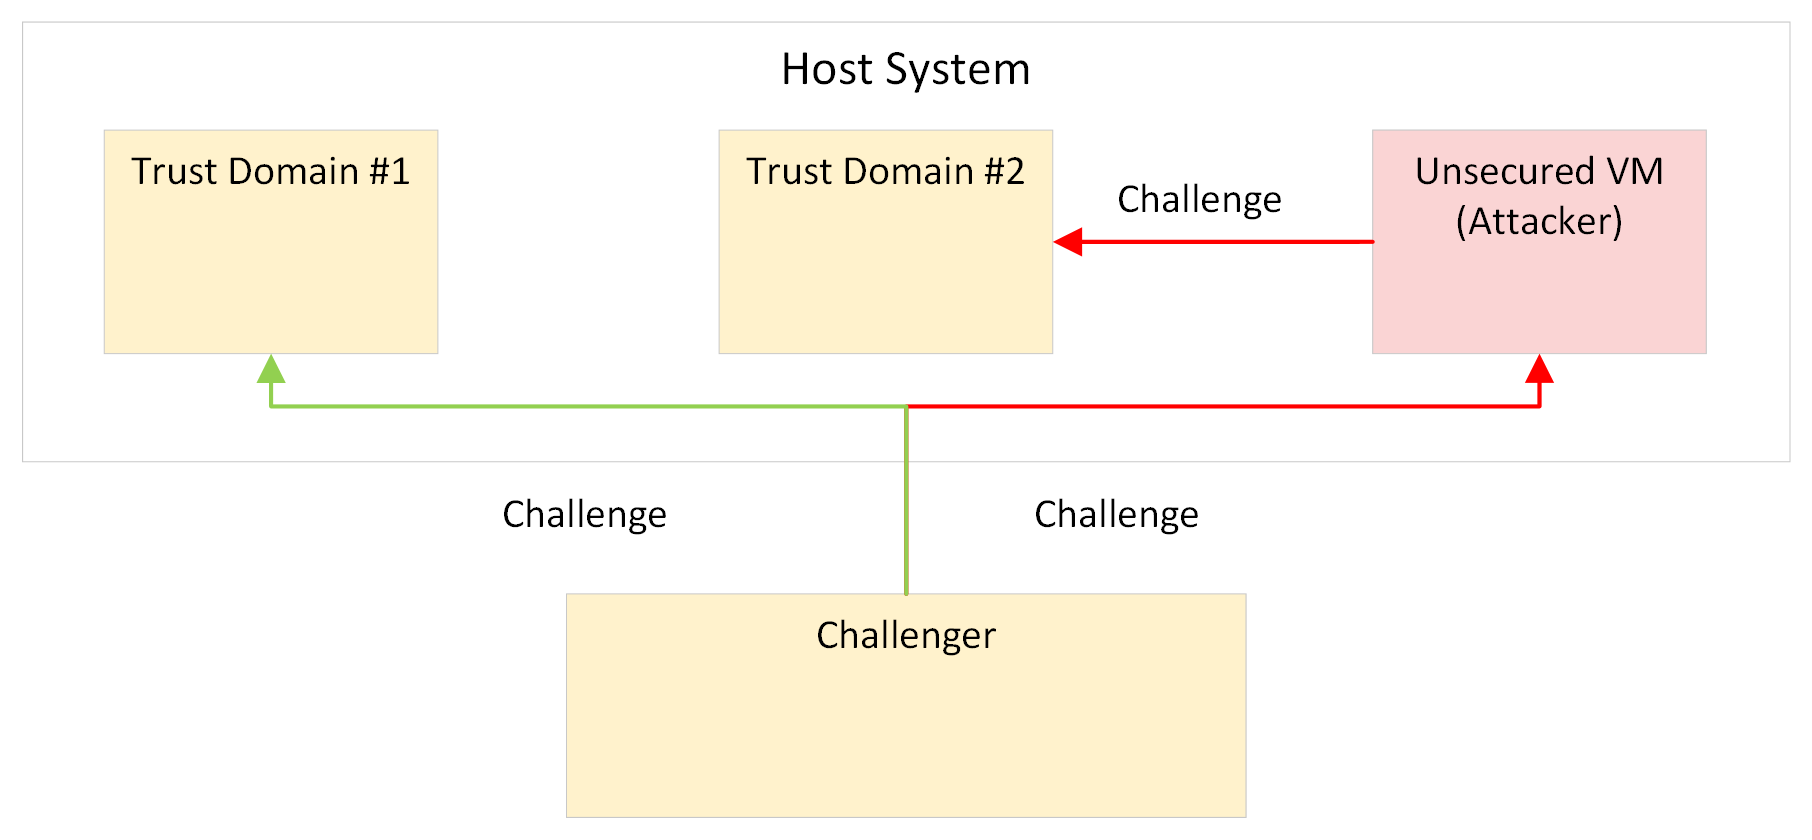
\includegraphics[width=.75\textwidth]{figures/Man-In-The-Middle.png} 
 \caption{Test}
 \label{fig:man_in_the_middle}
\end{figure}



\section{Security assumptions/solutions} \todo{title}
\todo{Public Key in Image -> MRTD Hash}
\todo{How to verify MRTD}

Going forward I propose three different ways to establish a secure connection, which get increasingly more complex, while reducing security assumptions and increasing adherence to best practices.

\myparagraph{Verifying the TD identity from a quote}

\label{Identity}
Similarly to SGX, with TDX the quote contains information on the startup environment of the TD. The Measurement of Trust Domain (MRTD) registers contain information on the initial state of the TD immediately after startup \cite{DCAP}. The Runtime Measurement Registers (RTMR) are written during the runtime, Intel recommends writing information about the virtual firmware configuration in RTMR[0] and information about the OS kernel and boot parameters in RTMR[1] \todo{Does DCAP verify those?}. Additionally the Quote can contain informal data in the \textbf{REPORTDATA} field, which could for example contain hashes about the current state of the filesystem or a nonce. The developer has to compare the expected state of the TD with the real state themself.

\subsection{Establishing a secure connection to the TD}
\label{Establishing_a_secure_connection}
\todo{Das geht nicht}After creation the TD contains a previously supplied public key. This public key can either be put into the image before creation or after. If this is done after, this means that the cloud provider has unmonitored acces to the TD and security is not guaranteed, this can be retraced by comparing the startup measurements of the TD with self calculated ones. If these match an empty image, there is a backdoor, if they match an image with just your public key in it, then the image is verified and SSH access to that image can only be done by you. This also means that it is no longer possible to fake the man in the middle attack in Figure \ref{fig:man_in_the_middle} because the attacker, would not have access to the same TD. This form of secure communication relies on the fact that only one public key is in the TD and thus the initial communication channel is secure. If somehow the initial communication channel can be compromised this is no longer secure. While theoretically secure, this relies on the assumption that the public key is not extractable from the image. QEMU and by extension TDX uses .qcow2 images, which can be encrypted and using a key management service, which is an additional trusted party, be decrypted on startup. If done using a cloud provider, they have to support this 
According to \cite{cheng_intel_2023} TDX and SGX can establish secure channels via SSL in a similar way:
In a typical scenario, when a client negotiates a secure channel with a server running in a TD, it aims to ensure a connection with a server that has been properly instantiated. The server, acting as an attester, generates a pair of ephemeral public and private keys. It calculates the hash of the public key and creates a TD report that includes this hash as the \textbf{REPORTDATA}. The server then requests a quote of the report and generates a self-signed certificate with the quote embedded in it. This self-signed certificate is provided as the server certificate in the TLS handshake protocol. Upon receiving the server certificate, the client, acting as the challenger, verifies the signatures on the certificate and validates the embedded quote, including the measurements. The client also checks if the quote includes the hash of the public key, as this associates the key with the TD. This contains the assumption that the client can verify the TD identity from the Quote \ref{verify_identity}. When establishing a secure channel, both the client and server can assume the roles of attester and verifier. This enables endpoints running in TDs to authenticate each other mutually by validating TDs\cite{knauth_integrating_2019}. Issues arising from self-signed certificates, the certificate size and similar are discussed as well, with all of them  having solutions. This form of secure communication relies on certificate authorities and can thus also work if the initial communication channel is compromised. Although the latter can mean that the entire TD can be compromised which invalidates other security assumptions. They thus have similar security assumptions and guarantees.

\todo{TD migration + Cloud provider availability promises, how is it done?}

\chapter{Implementation}

\section{Setting up a TDX VM on a new machine}
\label{ch:SettingUpTDX}
Intel supplies documents for a quick setup of TDX machines and TDs. In this section, \cite{noauthor_white_nodate} will be used as a reference. Intel internally supplies additional documents as well and code from there will be replicated here. The Server was supplied as an Intel DevCloud bare-metal machine with two Intel XEON 8490h processors with 60 cores respectively. Setting up Intel DevCloud and Trusted Domain for the first time took the better part of a week. The versioning in the different internal guides was off, which lead to an unusable Kernel, which was only fixed by complete reinstall. The version used in the end was 2023ww22 from may 2023. The guest image was created using the Intel tdx-tools tool for guest image creation\url{https://github.com/intel/tdx-tools/blob/tdx-1.5/build/ubuntu-22.04/guest-image/create-ubuntu-image.sh}.
This installs all the necessary kernel components to the images, as well as checking the respective hashes. Next the host kernel has to be patched. This requires downloading the correct packages from the Intel open source directory and then simply creating a patched kernel. Next TDX can be enabled and booted up using the newly patched kernel. To enable the possibility of attestation, the kernel needs Intel SGX Data Center Attestation Primitive (DCAP), which can also be installed from the Intel open source directory or downloaded from Github. We also need an implementation of the Provisioning Certification Caching Service, which Intel provides a reference implementation of, which can also be found in the Intel open source directory. Lastly, the Quote Generation Service contained in the SGX SDK must be installed. Now the Guest TD can be booted up. For this the following QEMU parameters were used:

\begin{itemize}
    \item \todo{QEMU Parameters}
\end{itemize}

\section{Benchmark Results}

\todo{General Benchmark results}
The Benchmark results using distilBERT-base-uncased show a small performance loss of 2\% from a TD VM to a Non-TD VM. The performance difference fluctuates between the non-TD VM being 3\% slower on the long sentence array transformer pipe to being 5\% faster on the long sentence AMX pipe. Half the benchmarks did not have a t-value that make them significant. For this test the 30 run times were run 3 times for a total of 90 test runs per benchmark. The AMX variant was on average 29\% faster with the differences ranging from 19\% to 50\% faster.
These differences can be seen using MAD and mean and standard deviation, meaning they are not only due to outliers. The first benchmarks had the TD VM about 18\% faster on average. This unexpected result meant running the tests two more times to remove any potential noises in the system. These closed the gap overall but only one suite had the expected outcome of the Non-TD VM running faster. See \ref{sec:appendix:benchmarks:bert} for the full results and \todo{add online archive for .json}.

The benchmark results using RoBERTa show a small performance loss of on average 1\% from a non-TD VM to a TD VM. The performance differs from about 5\% faster to 5\% slower. Each result was checked for significance using Student’s two-sample, two-tailed t-test with an alpha equal to 0.95. The absolute t-values range from 3.79 to 11.28. With 30 runs per test this results in p-values far below 0.01. Every result except 2 was faster on non-TD VMs. The AMX accelerated pipe was faster on the TD vm on the short sentence array and long sentences\todo{why}. So while theses tests are statistically significant the difference in speed is not significant for real-world applications. AMX vs Non-AMX showed a speed increase of about 30\% in this benchmark, this is in line with the expected 1/3 speed increase.
The full Benchmark results can be found in the Appendix \ref{sec:appendix:benchmarks:roberta}.

Both of the previous tests were done using an additional layer using a QEMU VM. Running the same benchmarks on the Host system directly averages an improvement of about 10\%. 
Due to the small margin between non-TD VMs and TD VM it was decided to test what disabling all TDX-related BIOS settings \cite{getting-started} would have as an impact. This showed a significant speedup of on average 24\% using distillbert and 44\% using Roberta. The highest speed-up with 78\% was observed on the short-sentence array using Roberta. The difference was measurably slower using the AMX pipe with the distilbert TDX-enabled AMX pipe on the long-sentence being 5\% faster even. This difference was still inside the standard deviation, so could reasonably be explained with variations in testing. On average the non-AMX benchmarks were 53\% faster using distillbert and 71\% faster using Roberta. Figure \ref{fig:distillbertMADNONAMX} clearly shows the speed difference after disabling TDX in the BIOS. 
\begin{figure}
   \centering
       \includegraphics[width=.95\textwidth]{figures/distillbertMAD.png} 
 \caption{Test}
 \label{fig:distillbertMADNONAMX}
\end{figure}
On the other hand Figure \ref{fig:distillbertMADAMX} shows no measurable speed difference after disabling TDX using the AMX-enabled Benchmarks. 
\begin{figure}
   \centering
       \includegraphics[width=.95\textwidth]{figures/distillbertMADAMX.png} 
 \caption{Test}
 \label{fig:distillbertMADAMX}
\end{figure}
The AMX benchmarks were, using the geometric mean, similar in speed using distillbert, with a difference that was not statistically significant. The AMX benchmarks using Roberta were about 21\% faster \todo{Roberta AMX results}. The overall speed-up was measurably faster than the initial observed AMX speedup, which indicates that this is not due to the omission of AMX in general but something different but having no speed-up using AMX with distillbert was an interesting result. \todo{herausfinden warum}
All prior tests were done using Ubuntu 22.04 and the next were done using Ubuntu 23.10 (from here on Ubuntu 23), because of instability issues. Rerunning the same tests using Ubuntu 23 the observed speed-up from a TD to TDX disabled diminished to just about 3\% with just TDX disabled and then an additional 3\% with memory-encryption disabled as well. These differences were small but the MAD on the measurements was even smaller, as can be seen in Figure \ref{fig:distillbertAMXUbuntu23} \ref{fig:distillbertAMXUbuntu23}. 
\begin{figure}
   \centering
       \includegraphics[width=.95\textwidth]{figures/inferencedistillberMADUbuntu23AMX.png} 
 \caption{Distillbert Inference times on Ubuntu 23 and Sapphire Rapid CPUs.}
 \label{fig:distillbertAMXUbuntu23}
\end{figure}
A further examination was conducted on discernible execution time differences using a profiler on Ubuntu 23, but with just an eight percent speed difference, there wasn't much to observe. \todo{Profiler Analyse} Minus the speed overhead of the profiler which was measured to be about 10 seconds, no matter the platform, the execution took between 77 and 85 seconds, with the highest being TDX and memory encryption bypass enabled, which supposedly speeds up calculations, so assuming no impact here, the margin of error has to be at least the difference between memory encryption bypass enabled and disabled benchmarks, which is about two seconds or 2.5 percent. So no useful overall differences can be observed but some internal methods display significant differences. Intels Extension For Pytorch (IPEX) optimizer copy method saw timing increases of up to 400\%, this seems to be entirely due to activating TDX, as without TDX the timings were all within one percent of each other, enabling TDX without memory bypass increased this time by about 100\% and enabling bypass increases this a further 250\%. Total times for this IPEX optimization instruction can be seen in \ref{tab:IpexOpti}. The IPEX "replacement" method for linear transformation which takes most of the calculations shows small speed differences of about 5\% - in line with the rest. Almost all of the remaining speed differences came from basic linear transformation as well as the other methods called by the models. They show speed increases of about 5\% each.
Having a look at the profiler results on the Azure cloud there are no clear results on overall speed but noticeably the IPEX copy and optimize instructions were once again measurably slower on the TD compared to a non-TD VM the optimization took about 20\% longer on the TD. This slow down is almost completely due to the time PyTorches clone function takes, which saw increases of 1000\% in total and per call time. Memory encryption itself had close to no impact on the speed here. Neither did the Memory Encryption Bypass. Looking into the implementation of this function this is not expected. Clone creates shallow copies of a tensor, with the lower hierarchy memory being shared. With both the original and the copy being situated inside the TD, this should have at most the same overhead as raw memory access which is outlined in \ref{tab:MemoryAccessSpeed}.
\begin{table}
\centering
\resizebox{\textwidth}{!}{%
\begin{tabular}{ m{0.2\textwidth} m{0.2\textwidth} m{0.2\textwidth} m{0.2\textwidth} m{0.2\textwidth} m{0.2\textwidth}}
\toprule
& TD with ME Bypass & TD without ME Bypass & No-TD with ME & No-TD with ME Bypass & No Memory Encryption \\
\midrule
IPEX optimize total time & 1.21s & 0.597s & 0.28s & 0.278s & 0.284s \\
\midrule
PyTorch clone method & 1.01s & 0.397s & 0.079s & 0.077s & 0.077s \\
\bottomrule
\end{tabular}
}
\caption{Comparison of different timings of IPEX optimization method}
\label{tab:IpexOpti}
\end{table}

Looking further into Host and Guest implementations of TDX on specific Ubuntu versions was deemed too much for this thesis.

\subsection{Benchmarking TDX parts}

As stated in the previous section there were significant speed differences between having TDX enabled and disabled in the Bios but basically none when TDX was enabled in the Bios but disabled in the VM. Further investigations into what causes these speed-ups were thus necessary. As stated in \ref{sec:tdxBuildingBlocks} there were essentially three functionalities that could be tested independently from TDX:
\begin{itemize}
    \item Total Memory Encryption 
    \item Intel VT, virtualization features
    \item Intel SGX
\end{itemize}

They were tested in the order outlined here.
For Total Memory Encryption, TDX and SGX were disabled, while Intel VT remained turned on. Stream \cite{Stream} and "PerformanceTest" \url{PerformanceTest} were used for benchmarking. Stream is the de facto standard for memory speed testing and PerformanceTest is a commonly used proprietary tool used to compare memory access. Using PerformanceTest there were small but measurable differences in latency of about 5\% and 2.5\% for reading speed. The Writing speed remained within 1\% of each other
\begin{table}
\centering
\resizebox{\textwidth}{!}{%
\begin{tabular}{ m{0.37\textwidth} m{0.25\textwidth} m{0.25\textwidth} m{0.13\textwidth}}
\toprule
Memory Benchmark Type & Memory encryption activated & Memory encryption deactivated & Difference \\
\midrule
Memory Allocation MB/s & 32445.11 & 33258.94 & 2.5\% \\
\midrule
Memory Read Cached MB/s & 27683.36 & 28148.14 & 1.6\% \\
\midrule
Memory Read Uncached MB/s & 10879.98 & 11123.77 & 2.2\% \\
\midrule
Memory Write Medium MB/s & 9592.82 & 9549.92 & -0.4\% \\
\midrule
Memory Write Threaded MB/s & 400550.9 & 411297.5 & 2.6\% \\
\midrule
Memory Latency ns & 64.3 & 61.4 & -4.5\% \\
\bottomrule
\end{tabular}
}
\caption{Results of Performancetests memory benchmark}
\label{tab:MemoryAccessSpeed}
\end{table}

With Stream, everything was tested disabled, just Memory Encryption enabled, and TDX completely enabled, and all three were within two percent of one another, with the encrypted memory being slightly faster than the other two. These results are most likely due to background noise of the system. \ref{fig:STREAM full results}

\begin{table}[]
    \centering
    \resizebox{\textwidth}{!}{%
    \begin{tabular}{m{0.2\textwidth} m{0.2\textwidth} m{0.2\textwidth} m{0.2\textwidth} m{0.2\textwidth} m{0.2\textwidth}}
    \hline
        Function & Best Rate MB/s Encrypted & Best Rate MB/s TDX enabled & Best Rate MB/s unencrypted & Best Rate Legacy VM MB/s & Best Rate TD MB/s \\ \hline
        Copy: & 292927.7 & 296714.7 & 292686.3 & 228281.2 & 209348.5979 \\ \hline
        Scale: & 291833.5 & 296603.3 & 293131.2 & 225828 & 206950.9938 \\ \hline
        Add: & 324643.9 & 318742.3 & 317304.6 & 250686.5 & 221401.8875 \\ \hline
        Triad: & 315635.1 & 329435.5 & 314132 & 232469.4 & 225711.5192 \\ \hline
        Normalized Geometric Mean & 1.418 & 1.437 & 1.410 & 1.085 & 1.000 \\ \hline
    \end{tabular}
    }
    \caption{Comparison of Memory Access speed using STREAM for various Non-VM settings as well as legacy VMs and TD}
\end{table}

\subsection{Security Attestation}

Attestation was not implemented or usable on the Intel Developer Cloud. Verifying usage of TDX was thus relying on the Linux Kernel itself as well as Bios settings made by the user via an SSH connection. Without attestation the security benefits were theoretically not given. This was accepted as having bare-metal access meant being able to verify TDX activation directly.


\subsection{Setting up the benchmarks}
\label{sec:SecondContent:SecondSection}

The benchmark will be run in Python, as it is the most commonly used programming language in natural language processing. The benchmarks will predominantly be an inference benchmark using distillBERT and roBERTa-base, the code can be found in the appendix \ref{app:BenchmarkCode}. All benchmarks will be run using the same image on their own QEMU KVM with 32 Cores and 64GB of RAM on a machine containing 2 Intel Xeon 8490H with each 60 cores @1.90 Ghz, except if stated otherwise. The setup and boilerplate code can be found in the appendix aswell \ref{app:Setup}. Performance is measured with Pyperf and each test is run 30 times with the median and the standard deviation being shown.
For the inference Benchmark a short sentence with 16 tokens and a long sentence with 146 tokens were used. The long sentence was supposed to have 128 tokens but due to an oversight the sentence was a bit longer than initially thought. Additional more fine-grained benchmarks were done later on.


\chapter{Self-hosting vs Azure}

Hosting a TD on your premises does not offer useful benefits. A TD is supposed to protect against unauthorized access to the machine, the direct hardware. There are nonetheless steps that have to be done manually or via a trusted service. \todo{Issues with separation of concern and trust (Benny Video)}

\section{Attestation}
 \todo{Microsoft, as will most other cloud providers, offers a attestation verification service hosted by them. There are generally four ways how attestation can be done that have their pros and contras:}
\begin{table}
\centering
\resizebox{0.9\textwidth}{!}{%
\begin{tabular}{ m{0.3\textwidth} m{0.2\textwidth} m{0.2\textwidth} m{0.2\textwidth} m{0.2\textwidth}}
\toprule
& Cloud Provider Attestation Service & Application Vendor Attestation Service & Independent Trust Service (E.g. Intel Trust Authority) & Build-Your-Own Service with DCAP \\
\midrule
Seperation of responsibilities between verifier and infrastructure provider & No & Yes & Yes & Yes \\
\midrule
Consistency across SGX and TDX & Yes, if both are offered & Yes, if both are supported & Yes & Yes \\
\midrule
Consistent service across on-prem, hybrid, multi-cloud, and edge deployments & No & Possible but unlikely or limited & Yes & Yes\\
\midrule
Development Effort & Low & Low & Low & Medium \\
\bottomrule
\end{tabular}
}
\caption{Overview of 4 different Attestation Verification methods}
\label{tab:AttestationVerification}
\end{table}


\todo{- Intel Trust Authority can verify with expected measurements
- Microsoft Azure Attestation aswell, but Verification is in enclave but no code provided, answer is just JWT token with signature. MRSigner (Hash des Public Keys des Signers (Microsoft)) is returned, MREnclave (Hash des Codes) isn't.}


\subsection{Microsoft Azure Attestation}
This section will explain in detail how Microsoft Azure Attestation (MAA) can be used, the pitfalls and issues with it. Notably the fact that following the tutorial on \url{https://learn.microsoft.com/en-us/azure/confidential-computing/quick-create-confidential-vm-portal} does not actually create a functioning TD VM but MAA will not actually tell you this. Following this tutorial, it is also not explained how to choose between AMD SEV-SNP and Intel TDX. This decision is entirely up to the chosen VM size which can only be inferred by looking at press releases pertaining Intel TDX and the newly released VM sizes. The DC\textbf{e}sv5, DC\textbf{e}dsv5 and EC\textbf{e}sv5, EC\textbf{e}dsv5 use Intel Xeon CPUs, while DC\textbf{a}sv5, DC\textbf{a}dsv5 and EC\textbf{a}sv5, EC\textbf{a}dsv5 use AMD Threadripper CPUs. The difference between D-instances and E-instances is the ratio between VCPU cores and memory, with E-instances having more memory per core. With the VM created there are a couple of ways how to create a TD Quote for attestation and the Azure confidential-computing-cvm-guest-attestation library \url{https://github.com/Azure/confidential-computing-cvm-guest-attestation/tree/tdx-preview}. Building the tdx-attestation app and using the supplied maa\_config file, which does only contain three settings, results in an apparently successful attestation and a jwt token returned. The entire decoded token can be found in \ref{app:jwttoken} but here we will focus on some parts of the td quote body. \cite{dcap} contains short explanation for all registers, which I will expand on a bit. We know that this has to be TDX 1.5 because tdx\_mrseam is not filled with 0, which would indicate TDX 1.0. The TEE\_TCB\_INFO struct contains two measurements, which are expected to be non-zero, one that has to be 0 with TDX and one that can be either. The non-zero are MRSEAM and TEE\_TCB\_SVN, which are filled. The zero-filled one is MRSIGNERSEAM, which also passes. Lastly TD\_ATTRIBUTES can be either. Intels recommendation for runtime-measurement registers tdx\_rtmr0 and tdx\_rtmr1 are as follows: Rtmr0 stores the measurements for TD Virtual Firmware, these are influenced by tdvm launch parameters, such as memory size. Most importantly this is locked in during startup and thus not user controlled in a cloud environment. In the excerpt returned by MAA this is filled with 0. Rtmr1 has two different purposes, depending on the boot option for the VM. With a direct boot it stores the kernel measurements and cmdline, that is passed to the kernel. With a grub boot it stores the grub measurements. Both of those are once again locked-in during the VM startup and out of control of the user. The register returned by MAA is once again only filled with 0, which is in itself not a violation of any standard but odd. The virtual firmware Intel offers for use does follow these instructions, meaning the firmware in use is a custom one by Microsoft which overwrites these changes.
\begin{lstlisting}[language=json]
  "tdx_mrconfigid": "000000000000000000000000000000000000000000000000000000000000000000000000000000000000000000000000",
  "tdx_mrowner": "000000000000000000000000000000000000000000000000000000000000000000000000000000000000000000000000",
  "tdx_mrownerconfig": "000000000000000000000000000000000000000000000000000000000000000000000000000000000000000000000000",
  "tdx_mrseam": "360304d34a16aace0a18e09ad2d07d2b9fd3c174378e5bf108388079827f89ff62acc5f8c473dd40706324834e202946",
  "tdx_mrsignerseam": "000000000000000000000000000000000000000000000000000000000000000000000000000000000000000000000000",
  "tdx_mrtd": "024a32b070383331181619fa387cb4d55d1e38879f989933055ccad5bc2db795d1737b66205949d15469dc8c1ba7ab7b",
  "tdx_report_data": "c90f98ba8ab80c7b442b6b8eb30af54e0508077b11adb525af6dfbcc8714e52a0000000000000000000000000000000000000000000000000000000000000000",
  "tdx_rtmr0": "000000000000000000000000000000000000000000000000000000000000000000000000000000000000000000000000",
  "tdx_rtmr1": "000000000000000000000000000000000000000000000000000000000000000000000000000000000000000000000000",
  "tdx_rtmr2": "000000000000000000000000000000000000000000000000000000000000000000000000000000000000000000000000",
  "tdx_rtmr3": "000000000000000000000000000000000000000000000000000000000000000000000000000000000000000000000000",
  "tdx_seam_attributes": "0000000000000000",
  "tdx_seamsvn": 258,
  "tdx_td_attributes": "0000000000000000",
  "tdx_td_attributes_debug": false,
  "tdx_td_attributes_key_locker": false,
  "tdx_td_attributes_perfmon": false,
  "tdx_td_attributes_protection_keys": false,
  "tdx_td_attributes_septve_disable": false,
  "tdx_tee_tcb_svn": "02010600000000000000000000000000",
  "tdx_xfam": "e718060000000000",
\end{lstlisting}
To verify if the guest VM is actually a td we have to verify a couple of things. In the file /proc/cpuinfo there needs to be a flag for tdx\_guest, this was false. The CC Event Log ACPI Table \url{https://uefi.org/specs/ACPI/6.5/05_ACPI_Software_Programming_Model.html#cc-event-log-acpi-table} needs to contain CC Type 2 for TDX - this table was not even present, which is a violation of the efi specifications if this really is a trusted domain \url{https://uefi.org/specs/UEFI/2.10/38_Confidential_Computing.html#efi-cc-measurement-protocol}. The information from this would have been present in the rtmr0 register.\todo{Find out how ACPI Table looks like} Lastly a pipe called tdx\_guest, tdx-attestation or tdx-guest depending on the version should be present. These function as an interface to retrieve TDX-guest specific information\url{https://docs.kernel.org/virt/coco/tdx-guest.html}. It is used to retrieve the TDREPORT for the attestation, covering steps 2 and 8 in Fig\ref{fig:QuoteGeneration}.  This also was not present. This means that the Guest VM was neither a TDVM, nor is it compliant with other confidential computing VM standards. This itself does not make the hardware attestation from MAA impossible but makes it much more difficult to implement your own attestation. It appears that Microsoft recreated the tdx\_guest interface somewhere but does not tell the user how it was done or if it was done exactly the same way. The User now needs to recreate this pipe manually somehow. I tried to reuse one from another platform, which sadly was not compatible.
From Fig. \ref{fig:component-overview} this means that the TDX-Englightened OS is an unmodified OS.
\todo{verify https://ccthesisaaprovider.weu.attest.azure.net/certs }
Using the openID enpoint to get the certificates used, I verified the validity and signature of the token. 
\todo{verify chain of trust with intel service}


%%\todo{download qe3-logic, urts, enclave-common, ae-pce händisch von 01.org, ansonsten https://github.com/intel/SGXDataCenterAttestationPrimitives/tree/tdx_1.5_dcap/QuoteGeneration}
\begin{figure}
\centering
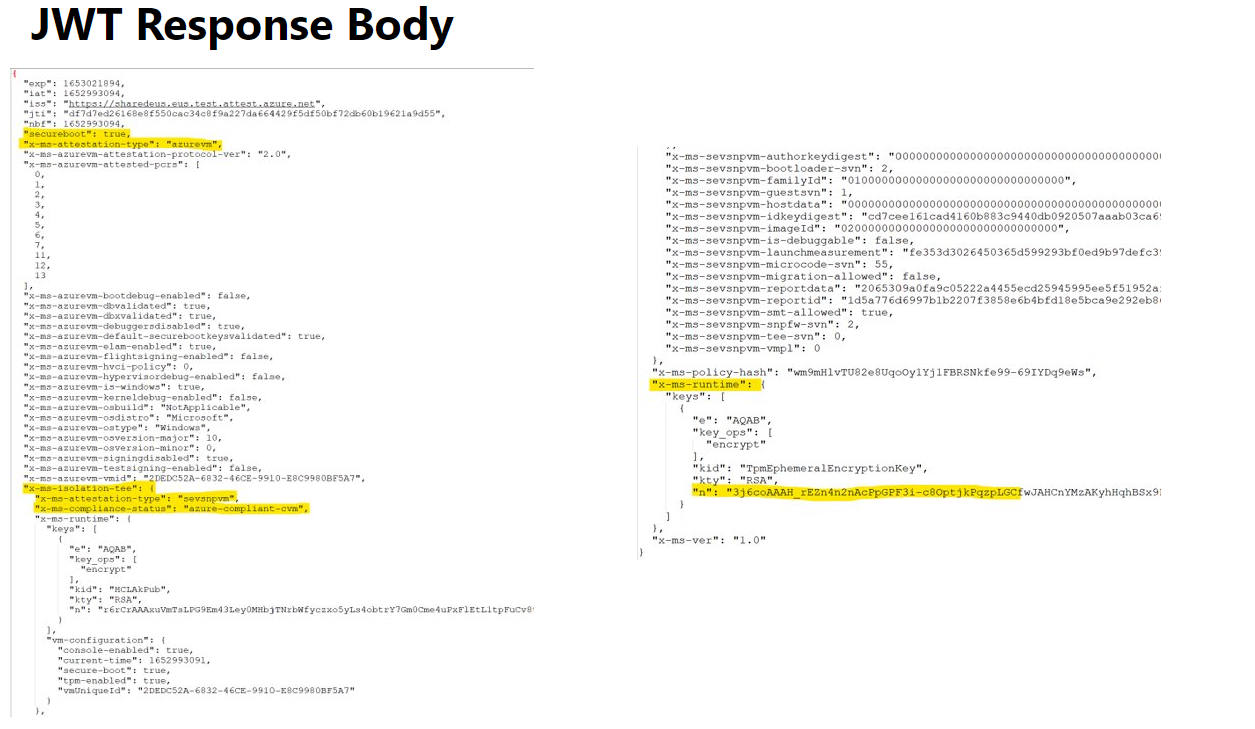
\includegraphics[width=\textwidth]{figures/JWT-response-token-azure-attestation.png}
\caption{Examplary JWT response token from \url{https://github.com/Azure/confidential-computing-cvm-guest-attestation/tree/main/cvm-attestation-sample-app}}
\label{fig:STREAM full results}
\end{figure}

MAA-Code zur Verfügung gestellt für "Government Customers"
- IAA, Application \& Intel kein Code, Build-Your-Own Service OSS und eigener Code
- Externe müssen DCAP verwenden, gleiche Schritte, Collateral von Intel wird auch benötigt



MAA attestaion verification is successful even without working TDX

Seperation of responsibility between verifier and infrastructure provider

Hosting your VMs bare metal on your own hardware will offer performance increases similar to the ones outlined in \ref{BenchmarkResults}. With security guarantees similar to the ones that TDX can offer. Even better if security to your premises is better.

\todo{Selbsthosten ergibt keinen Sinn}
\todo{Was für Vor und Nachteile gibt es? Performanceeinbußen}
\todo{Was muss ich noch selber machen in der Cloud? E.g. Attestation}
\todo{}


\section{Application Possibilities}

\todo{Wirklich sicher?}
\todo{Was ist der Nutzervorteil?}
\todo{Wie komplex ist die Nutzung?}
%% ---------------------
%% | / Example content |
%% ---------------------



\section{Outlook}

This thesis focused on simple TDX implementations. With TDX having been just released, most of those implementations are still in their infancy and problems are to be expected. Hopefully in the future some of those, that have been highlighted in this thesis and those that have not been will be fixed. Nonetheless there are still additional things that can be looked at. The implementation of TDX in Ubuntu 22 appears to cause instability issues and also performance defiencies compared to the implementation in Ubuntu 23. Having a deeper look at the differences between those two could grant significant improvements. Additionally comparisons between the different hardware Confidential Computing hardware providers are necessary to being able to make the decision for or against Confidential Computing. Additionally looking into the implementation of PyTorch to figure out why its copy function experiences such significant slowdown is advised. 

For the future Intel has planned on a cooperation with Nvidia to bring Confidential Computing and AI closer together \url{https://community.intel.com/t5/Blogs/Products-and-Solutions/Security/Intel-Nvidia-Collaborate-to-Deliver-Confidential-AI-Solutions/post/1500066}. With the release of Intel attestation for Nvidia hardware to be planned in the first half of 2024, confidential computing on GPU hardware could be a possibility. Intel and Nvidia have yet to release architecture specifications for their collaboration but their security promises and assumptions will have to be tested then. If implementation could be simplified for the average user this could be a great step into the right direction for data security. The dangers of dedicated GPUs and the possible performance losses with establishing a secure communication between CPU and GPU are a challenge that will have to be solved first. Silberstein et al. highlighted the dangers of insecure communication and other problems with dedicated GPUs in their 2020 paper \cite{Silberstein_GPUAttack}.

Additionally this thesis was limited in regard to the amount of performancetesting that was feasible. More I/O heavy workloads and even some GPU-bound workloads could be tested. Implementing ways to calculate on a non-trusted GPU, while maintaining data confidentiality is still an ongoing line of research, which could be even more interesting in the future, but it still has security and performance problems, compare \cite{Monique Ogburn} and \cite{Baiyu Li} for more information on this.


\todo{Integration with GPUs, FPGAs, TPUs,...}
